\documentclass [10pt]{article}
\textheight	8.7in
\textwidth	6.5in
\topmargin	    0in
\oddsidemargin  0in
\evensidemargin 0in
\baselineskip 15pt

\usepackage[top=1in, bottom=1in, left=1in, right=1in]{geometry}

\usepackage{amssymb,amsmath,amstext}
\usepackage{amsfonts}
\usepackage{mathtools}
\usepackage{forest}
\usepackage{tikz}
\usetikzlibrary{automata,arrows,calc,positioning}

\begin{document}
\title{Theory of Computation Assignment no. 8}
\author{Goktug Saatcioglu}
\date{}
\maketitle
\begin{enumerate}
	\item[\textbf{(1)}]
	\begin{enumerate}
		\item[a.]The simple PDA $M^{\prime}$ such that $L(M)=L(M^{\prime})$ is given below.\\
		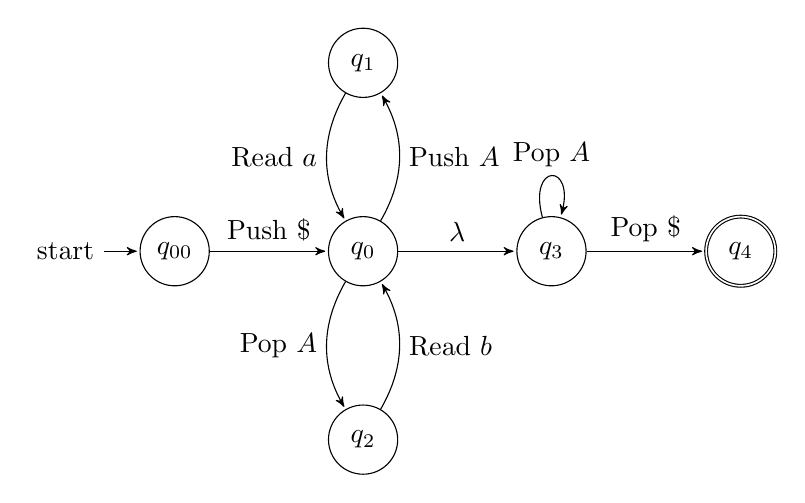
\begin{tikzpicture}[baseline=(q_0.north),>=stealth',shorten >=1pt, auto,node distance=1.5cm,align=center]
			\node[state,initial] (q_0) {$q_{00}$};
			\node[state] [right=of q_0] (q_1) {$q_{0}$};
			\node[state] [above=of q_1] (q_2) {$q_{1}$};
			\node[state] [below=of q_1] (q_3) {$q_{2}$};
			\node[state] [right=of q_1] (q_4) {$q_{3}$};
			\node[state,accepting] [right=of q_4] (q_5) {$q_{4}$};
			\path[->]
				(q_0) edge node {Push $\$$} (q_1)
				(q_1) edge [bend right] node [right] {Push $A$} (q_2)
				(q_2) edge [bend right] node [left] {Read $a$} (q_1)
				(q_1) edge [bend right] node [left] {Pop $A$} (q_3)
				(q_3) edge [bend right] node [right] {Read $b$} (q_1)
				(q_1) edge node {$\lambda$} (q_4)
				(q_4) edge [loop above] node {Pop $A$} ()
				(q_4) edge node {Pop $\$$} (q_5);
		\end{tikzpicture}\par
		Where $q_{00}$ is the intial state before the shielding symbol is pushed onto the stack, $q_{0}$ is $q_{0}$ from $M$, $q_{1}$ is the intermediary step in the upper loop of $M$, $q_{2}$ is the inermediary step in the lower loop of $M$, $q_{3}$ is the stack empyting step and $q_{4}$ is the accepting state once the stack is empty.
		\item[b.]A derivation tree for the word $w=abaab$ is given below.\\
		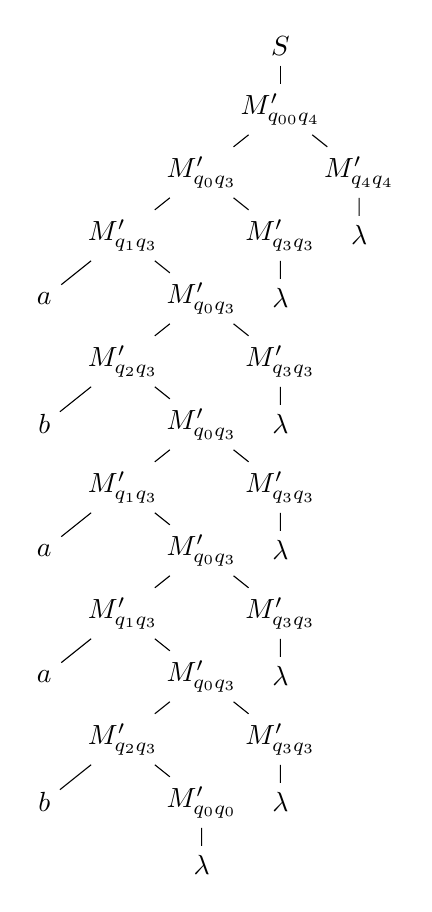
\begin{tikzpicture}[sibling distance=20mm,level distance=8mm
		]
			\node {$S$}
			child { node {$M^{\prime}_{q_{00}q_{4}}$}
			child { node {$M^{\prime}_{q_{0}q_{3}}$} 
			child { node {$M^{\prime}_{q_{1}q_{3}}$} 
			child { node {$a$} }
			child { node {$M^{\prime}_{q_{0}q_{3}}$}
			child { node {$M^{\prime}_{q_{2}q_{3}}$}
			child { node {$b$} }
			child { node {$M^{\prime}_{q_{0}q_{3}}$} 
			child { node {$M^{\prime}_{q_{1}q_{3}}$}
			child { node {$a$} } 
			child { node {$M^{\prime}_{q_{0}q_{3}}$} 
			child { node {$M^{\prime}_{q_{1}q_{3}}$}
			child { node {$a$} } 
			child { node {$M^{\prime}_{q_{0}q_{3}}$} 
			child { node {$M^{\prime}_{q_{2}q_{3}}$} 
			child { node {$b$} }
			child { node {$M^{\prime}_{q_{0}q_{0}}$} 
			child { node {$\lambda$} } } } 
			child { node {$M^{\prime}_{q_{3}q_{3}}$} 
			child { node {$\lambda$} } } } } 
			child { node {$M^{\prime}_{q_{3}q_{3}}$} 
			child { node {$\lambda$} } } } } 
			child { node {$M^{\prime}_{q_{3}q_{3}}$} 
			child { node {$\lambda$} } } } } 
			child { node {$M^{\prime}_{q_{3}q_{3}}$} 
			child { node {$\lambda$} } } } } 
			child { node {$M^{\prime}_{q_{3}q_{3}}$} 
			child { node {$\lambda$} } } }
			child { node {$M^{\prime}_{q_{4}q_{4}}$} 
			child { node {$\lambda$} } } }
		;
		\end{tikzpicture}
	\end{enumerate}
	\item[\textbf{(2)}]The transformation of the CFG into a PDA is given below. We begin by defining the PDA with the main state and then define the transition in and out of main.\\
	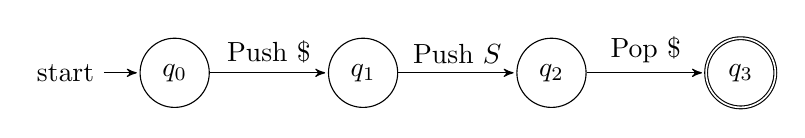
\begin{tikzpicture}[baseline=(q_0.north),>=stealth',shorten >=1pt, auto,node distance=1.5cm,align=center]
		\node[state,initial] (q_0) {$q_{0}$};
		\node[state] [right=of q_0] (q_1) {$q_{1}$};
		\node[state] [right=of q_1] (q_2) {$q_{2}$};
		\node[state,accepting] [right=of q_2] (q_3) {$q_{3}$};
		\path[->]
			(q_0) edge node {Push $\$$} (q_1)
			(q_1) edge node {Push $S$} (q_2)
			(q_2) edge node {Pop $\$$} (q_3);
	\end{tikzpicture}\par
	Here $q_{0}$ is the initial state, $q_{1}$ is the state with the shielding state, $q_{2}$ is main where we begin by pushing $S$ and $q_{3}$ is the accepting state. Next, for each rule we show a set of transition out from main and back into main. We begin with the rule $S\rightarrow aS^{a}S$.\\
	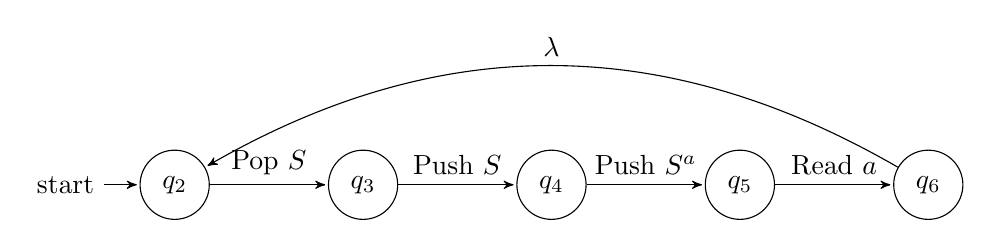
\begin{tikzpicture}[baseline=(q_0.north),>=stealth',shorten >=1pt, auto,node distance=1.5cm,align=center]
		\node[state,initial] (q_0) {$q_{2}$};
		\node[state] [right=of q_0] (q_1) {$q_{3}$};
		\node[state] [right=of q_1] (q_2) {$q_{4}$};
		\node[state] [right=of q_2] (q_3) {$q_{5}$};
		\node[state] [right=of q_3] (q_4) {$q_{6}$};
		\path[->]
			(q_0) edge node {Pop $S$} (q_1)
			(q_1) edge node {Push $S$} (q_2)
			(q_2) edge node {Push $S^{a}$} (q_3)
			(q_3) edge node {Read $a$} (q_4)
			(q_4) edge [bend right] node [above] {$\lambda$} (q_0);
	\end{tikzpicture}\par
	Here $q_{2}$ is main and the rest of the states is the derivation rule processed in reverse. Similarly, we write the transitions for the rule $S\rightarrow bS^{b}S$.\\
	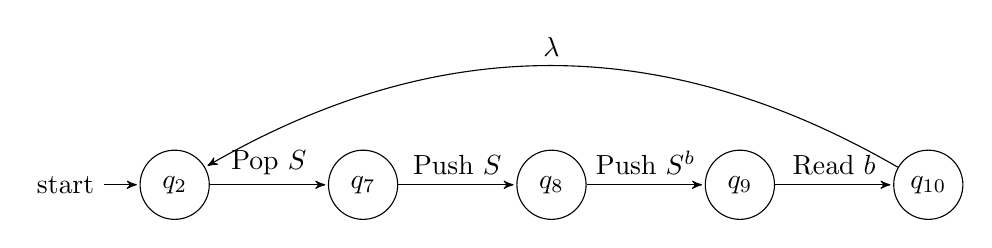
\begin{tikzpicture}[baseline=(q_0.north),>=stealth',shorten >=1pt, auto,node distance=1.5cm,align=center]
		\node[state,initial] (q_0) {$q_{2}$};
		\node[state] [right=of q_0] (q_1) {$q_{7}$};
		\node[state] [right=of q_1] (q_2) {$q_{8}$};
		\node[state] [right=of q_2] (q_3) {$q_{9}$};
		\node[state] [right=of q_3] (q_4) {$q_{10}$};
		\path[->]
			(q_0) edge node {Pop $S$} (q_1)
			(q_1) edge node {Push $S$} (q_2)
			(q_2) edge node {Push $S^{b}$} (q_3)
			(q_3) edge node {Read $b$} (q_4)
			(q_4) edge [bend right] node [above] {$\lambda$} (q_0);
	\end{tikzpicture}\par
	Again $q_{2}$ is main and we reverse process the derivation rules. Next, we write the derivation for the rule $S\rightarrow\lambda$ with $q_{2}$ as main.\\
	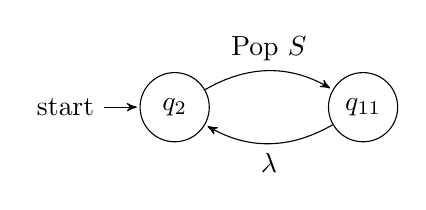
\begin{tikzpicture}[baseline=(q_0.north),>=stealth',shorten >=1pt, auto,node distance=1.5cm,align=center]
		\node[state,initial] (q_0) {$q_{2}$};
		\node[state] [right=of q_0] (q_1) {$q_{11}$};
		\path[->]
			(q_0) edge [bend left] node {Pop $S$} (q_1)
			(q_1) edge [bend left] node [below] {$\lambda$} (q_0);
	\end{tikzpicture}\par
	We then get two more derivations for the rule $S^{a} \rightarrow a\:|\:a^S{a}S^{a}$ with $q_{2}$ as main.\\
	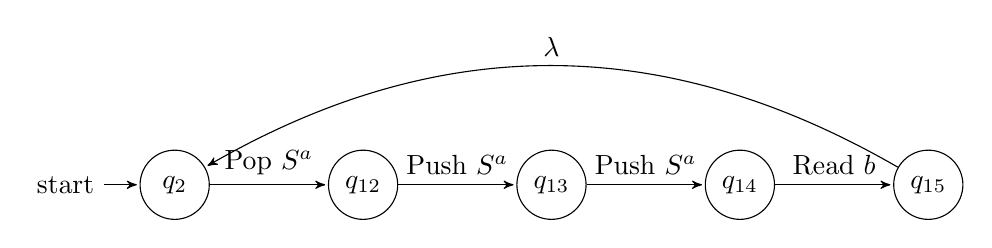
\begin{tikzpicture}[baseline=(q_0.north),>=stealth',shorten >=1pt, auto,node distance=1.5cm,align=center]
		\node[state,initial] (q_0) {$q_{2}$};
		\node[state] [right=of q_0] (q_1) {$q_{12}$};
		\node[state] [right=of q_1] (q_2) {$q_{13}$};
		\node[state] [right=of q_2] (q_3) {$q_{14}$};
		\node[state] [right=of q_3] (q_4) {$q_{15}$};
		\path[->]
			(q_0) edge node {Pop $S^{a}$} (q_1)
			(q_1) edge node {Push $S^{a}$} (q_2)
			(q_2) edge node {Push $S^{a}$} (q_3)
			(q_3) edge node {Read $b$} (q_4)
			(q_4) edge [bend right] node [above] {$\lambda$} (q_0);
	\end{tikzpicture}\par
	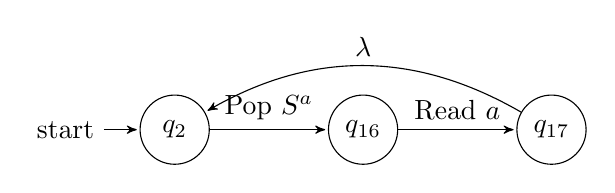
\begin{tikzpicture}[baseline=(q_0.north),>=stealth',shorten >=1pt, auto,node distance=1.5cm,align=center]
		\node[state,initial] (q_0) {$q_{2}$};
		\node[state] [right=of q_0] (q_1) {$q_{16}$};
		\node[state] [right=of q_1] (q_2) {$q_{17}$};
		\path[->]
			(q_0) edge node {Pop $S^{a}$} (q_1)
			(q_1) edge node {Read $a$} (q_2)
			(q_2) edge [bend right] node [above] {$\lambda$} (q_0);
	\end{tikzpicture}\par
	Finally, we get two more derivations for the rule $S^{b} \rightarrow b\:|\:a^S{b}S^{b}$ with $q_{2}$ as main.\\
	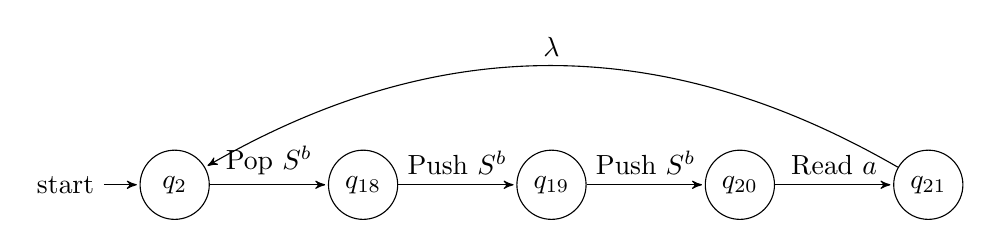
\begin{tikzpicture}[baseline=(q_0.north),>=stealth',shorten >=1pt, auto,node distance=1.5cm,align=center]
		\node[state,initial] (q_0) {$q_{2}$};
		\node[state] [right=of q_0] (q_1) {$q_{18}$};
		\node[state] [right=of q_1] (q_2) {$q_{19}$};
		\node[state] [right=of q_2] (q_3) {$q_{20}$};
		\node[state] [right=of q_3] (q_4) {$q_{21}$};
		\path[->]
			(q_0) edge node {Pop $S^{b}$} (q_1)
			(q_1) edge node {Push $S^{b}$} (q_2)
			(q_2) edge node {Push $S^{b}$} (q_3)
			(q_3) edge node {Read $a$} (q_4)
			(q_4) edge [bend right] node [above] {$\lambda$} (q_0);
	\end{tikzpicture}\par
	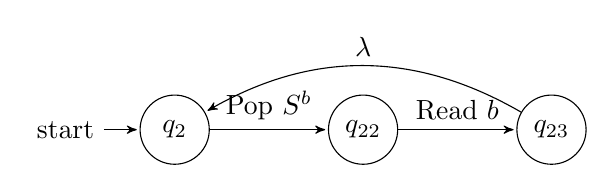
\begin{tikzpicture}[baseline=(q_0.north),>=stealth',shorten >=1pt, auto,node distance=1.5cm,align=center]
		\node[state,initial] (q_0) {$q_{2}$};
		\node[state] [right=of q_0] (q_1) {$q_{22}$};
		\node[state] [right=of q_1] (q_2) {$q_{23}$};
		\path[->]
			(q_0) edge node {Pop $S^{b}$} (q_1)
			(q_1) edge node {Read $b$} (q_2)
			(q_2) edge [bend right] node [above] {$\lambda$} (q_0);
	\end{tikzpicture}\par
	Thus, we have transformed the CFG into a PDA that accepts thesame language.
	\item[\textbf{(3)}]
	\begin{enumerate}
		\item[(a)]$L(P)=\{u\#v\:|\:u,v\in\{a,b\}^{*}\:\text{and}\:\#_a(u)-\#_b(u)=\#_a(v)-\#_b(v)\}$
		\item[(b)]A data-configuration sequence of an accepting computation path in $P$ for the word $w = abb\#abb$ is given below.
		\begin{align}
			\rightarrow(\lambda,q_{0},\lambda)&\rightarrow(\lambda,q_{1},\$)\rightarrow(a,q_{1},P\$)\rightarrow(ab,q_{1},\$)\rightarrow(abb,q_{1},N\$)\rightarrow(abb\#,q_{2},N\$)\dots\nonumber\\
			&\dots\rightarrow(abb\#a,q_{2},NN\$)\rightarrow(abb\#ab,q_{2},N\$)\rightarrow(abb\#abb,q_{2},\$)\rightarrow(abb\#abb,q_{3},\lambda)\nonumber
		\end{align}
		Here $q_{i}$ is the $i$-th state from the left.
		\item[(c)]The simple PDA $P^{\prime}$ such that $L(P)=L(P^{\prime})$ is given below.\\
		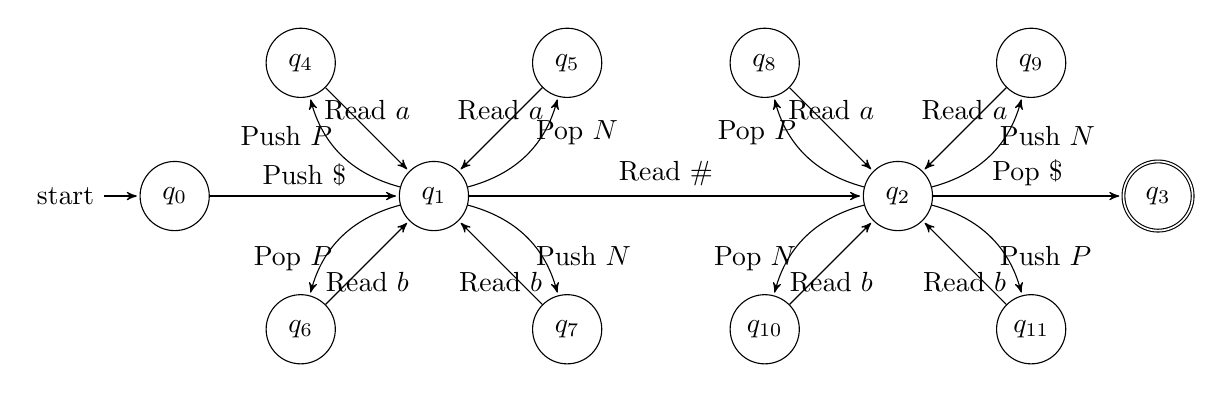
\begin{tikzpicture}[baseline=(q_0.north),>=stealth',shorten >=1pt, auto,node distance=1.5cm,align=center]
			\node[state,initial] (q_0) {$q_{0}$};
			\node[state] [right=2.4cm of q_0] (q_1) {$q_{1}$};
			\node[state] [right=5cm of q_1] (q_2) {$q_{2}$};
			\node[state,accepting] [right=2.4cm of q_2] (q_3) {$q_{3}$};
			\node[state] [above left=of q_1] (q_4) {$q_{4}$};
			\node[state] [above right=of q_1] (q_5) {$q_{5}$};
			\node[state] [below left=of q_1] (q_6) {$q_{6}$};
			\node[state] [below right=of q_1] (q_7) {$q_{7}$};
			\node[state] [above left=of q_2] (q_8) {$q_{8}$};
			\node[state] [above right=of q_2] (q_9) {$q_{9}$};
			\node[state] [below left=of q_2] (q_10) {$q_{10}$};
			\node[state] [below right=of q_2] (q_11) {$q_{11}$};
			\path[->]
				(q_0) edge node {Push $\$$} (q_1)
				(q_1) edge node {Read $\#$} (q_2)
				(q_2) edge node {Pop $\$$} (q_3)
				(q_1) edge [bend left] node [above left] {Push $P$} (q_4)
				(q_4) edge node [above] {Read $a$} (q_1)
				(q_1) edge [bend right] node [above right] {Pop $N$} (q_5)
				(q_5) edge node [above] {Read $a$} (q_1)
				(q_1) edge [bend right] node [below left] {Pop $P$} (q_6)
				(q_6) edge node [below] {Read $b$} (q_1)
				(q_1) edge [bend left] node [below right] {Push $N$} (q_7)
				(q_7) edge node [below] {Read $b$} (q_1)
				(q_2) edge [bend left] node [above left] {Pop $P$} (q_8)
				(q_8) edge node [above] {Read $a$} (q_2)
				(q_2) edge [bend right] node [above right] {Push $N$} (q_9)
				(q_9) edge node [above] {Read $a$} (q_2)
				(q_2) edge [bend right] node [below left] {Pop $N$} (q_10)
				(q_10) edge node [below] {Read $b$} (q_2)
				(q_2) edge [bend left] node [below right] {Push $P$} (q_11)
				(q_11) edge node [below] {Read $b$} (q_2);
		\end{tikzpicture}\par
		Here $q_{0}$, $q_{1}$, $q_{2}$ and $q_{3}$ are the states given by the PDA $P$ and the remaining states are the intermediary steps in the loops of $P$ where for example the left-top loop of $q_{1}$ which goes to $q_{4}$ is the left-top loop of $q_{1}$ in PDA $P$.
		\item[(d)]A derivation tree for the word $w=abb\#abb$ is given below.\\
		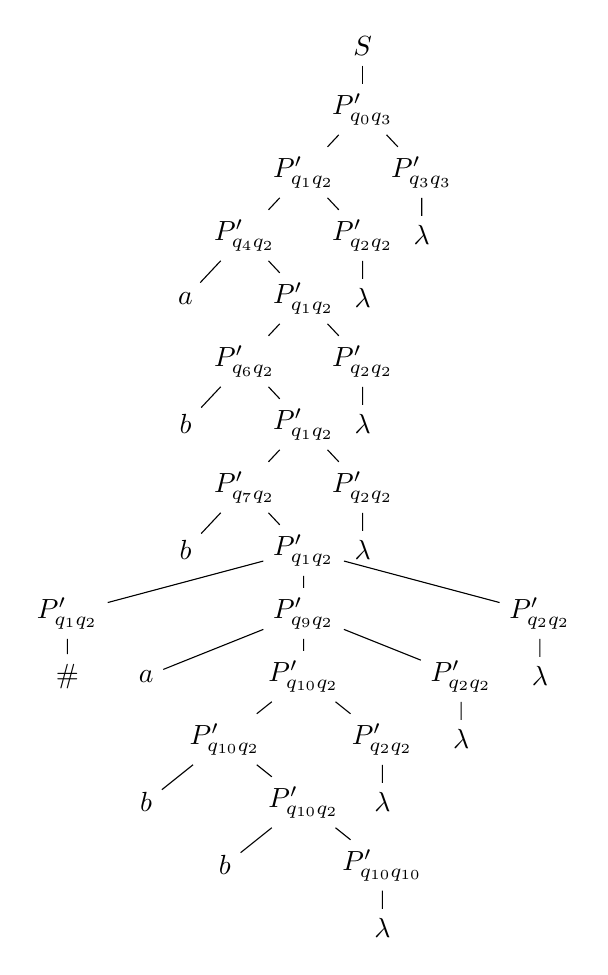
\begin{tikzpicture}[level 9/.style={sibling distance=30mm},level 10/.style={sibling distance=20mm},sibling distance=15mm,level distance=8mm
		]
		\node {$S$}
			child { node {$P^{\prime}_{q_{0}q_{3}}$} 
			child { node {$P^{\prime}_{q_{1}q_{2}}$} 
			child { node {$P^{\prime}_{q_{4}q_{2}}$}
			child { node {$a$} }
			child { node {$P^{\prime}_{q_{1}q_{2}}$}
			child { node {$P^{\prime}_{q_{6}q_{2}}$}
			child { node {$b$} }
			child { node {$P^{\prime}_{q_{1}q_{2}}$}
			child { node {$P^{\prime}_{q_{7}q_{2}}$}
			child { node {$b$} }
			child { node {$P^{\prime}_{q_{1}q_{2}}$} 
			child { node {$P^{\prime}_{q_{1}q_{2}}$} 
			child { node {$\#$} } }
			child { node {$P^{\prime}_{q_{9}q_{2}}$} 
			child { node {$a$} } 
			child { node {$P^{\prime}_{q_{10}q_{2}}$}
			child { node {$P^{\prime}_{q_{10}q_{2}}$} 
			child { node {$b$} }
			child { node {$P^{\prime}_{q_{10}q_{2}}$} 
			child { node {$b$} } 
			child { node {$P^{\prime}_{q_{10}q_{10}}$} 
			child { node {$\lambda$} } } } } 
			child { node {$P^{\prime}_{q_{2}q_{2}}$} 
			child { node {$\lambda$} } } } 
			child { node {$P^{\prime}_{q_{2}q_{2}}$} 
			child { node {$\lambda$} } } }  
			child { node {$P^{\prime}_{q_{2}q_{2}}$} 
			child { node {$\lambda$} } } } }
			child { node {$P^{\prime}_{q_{2}q_{2}}$} 
			child { node {$\lambda$} } } } }
			child { node {$P^{\prime}_{q_{2}q_{2}}$} 
			child { node {$\lambda$} } } } }
			child { node {$P^{\prime}_{q_{2}q_{2}}$} 
			child { node {$\lambda$} } } } 
			child { node {$P^{\prime}_{q_{3}q_{3}}$} 
			child { node {$\lambda$} } } }
		;
		\end{tikzpicture}
	\end{enumerate}
\end{enumerate}
\end{document}